\section{CQ2}

\begin{fancyquote}
    \textbf{Question:}\\
    How many CoAP resources in the local server received the same number of unique unsuccessful Confirmable POST and PUT requests?\\
    Assuming a resource receives $X$ different CON unsuccessful POST requests and $Y$ different CON unsuccessful PUT requests, how many resources have $X=Y$, with $X>0$?
    
    \vspace{0.1cm}
    \textit{!! Consider unsuccessful only if there is a response stating it is not successful !!}
\end{fancyquote}

\vspace{0.3cm}

\noindent
\begin{minipage}{\linewidth}
\subsection*{Isolate Unsuccessful Responses}
An "unsuccessful" response in CoAP means the server returned a Client Error (\texttt{4.xx}) or a Server Error (\texttt{5.xx}). Any response code between 128 and 191 is an explicit unsuccessful response.

\textbf{Filter:}
\begin{lstlisting}
ip.src == 127.0.0.1 && coap.code >= 128 && coap.code <= 191
\end{lstlisting}
This extracts just the tokens of all explicit error responses sent by the server and saves them to a text file.

\begin{figure}[H]
    \centering
    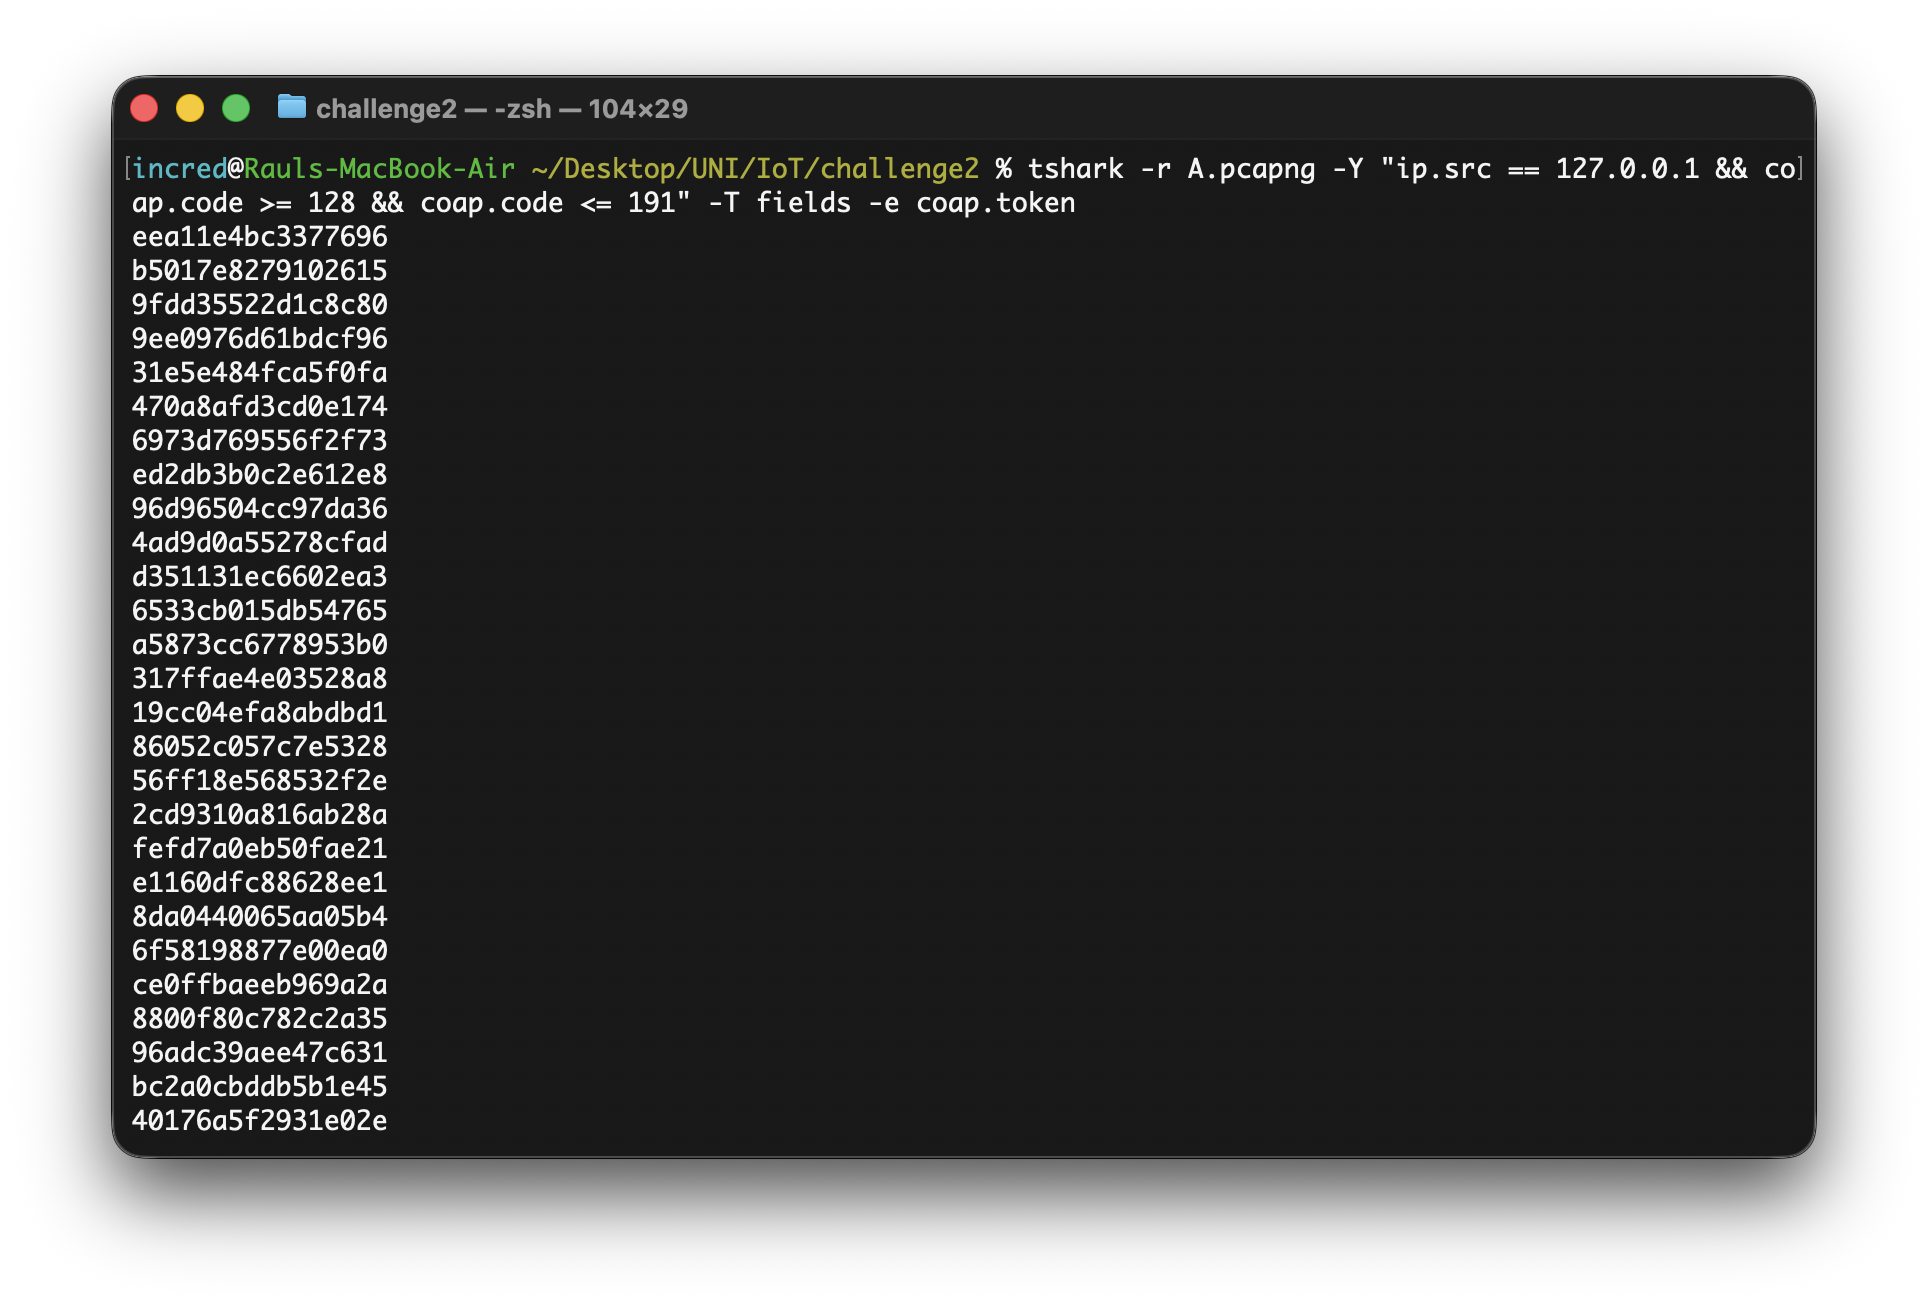
\includegraphics[width=0.75\linewidth]{images/cq2-unsuccessful.png}
\end{figure}
Output is saved in \textbf{\texttt{unsuccessful\_tokens.txt}}
\end{minipage}

\vspace{0.5cm}

\subsection*{Extract CON POST and CON PUT Requests}
We need to capture all Confirmable (\texttt{coap.type == 0}) POST (\texttt{coap.code == 2}) and PUT (\texttt{coap.code == 3}) requests directed at the server. We must extract both the Token (to match with the errors) and the URI Path (which represents the resource).

\begin{figure}[H]
    \centering
    \begin{minipage}[t]{0.48\textwidth}
        \textbf{Extract CON POST requests:}
\begin{lstlisting}
ip.dst == 127.0.0.1 && 
coap.type == 0 && coap.code == 2
\end{lstlisting}
        \vspace{0.1cm}
        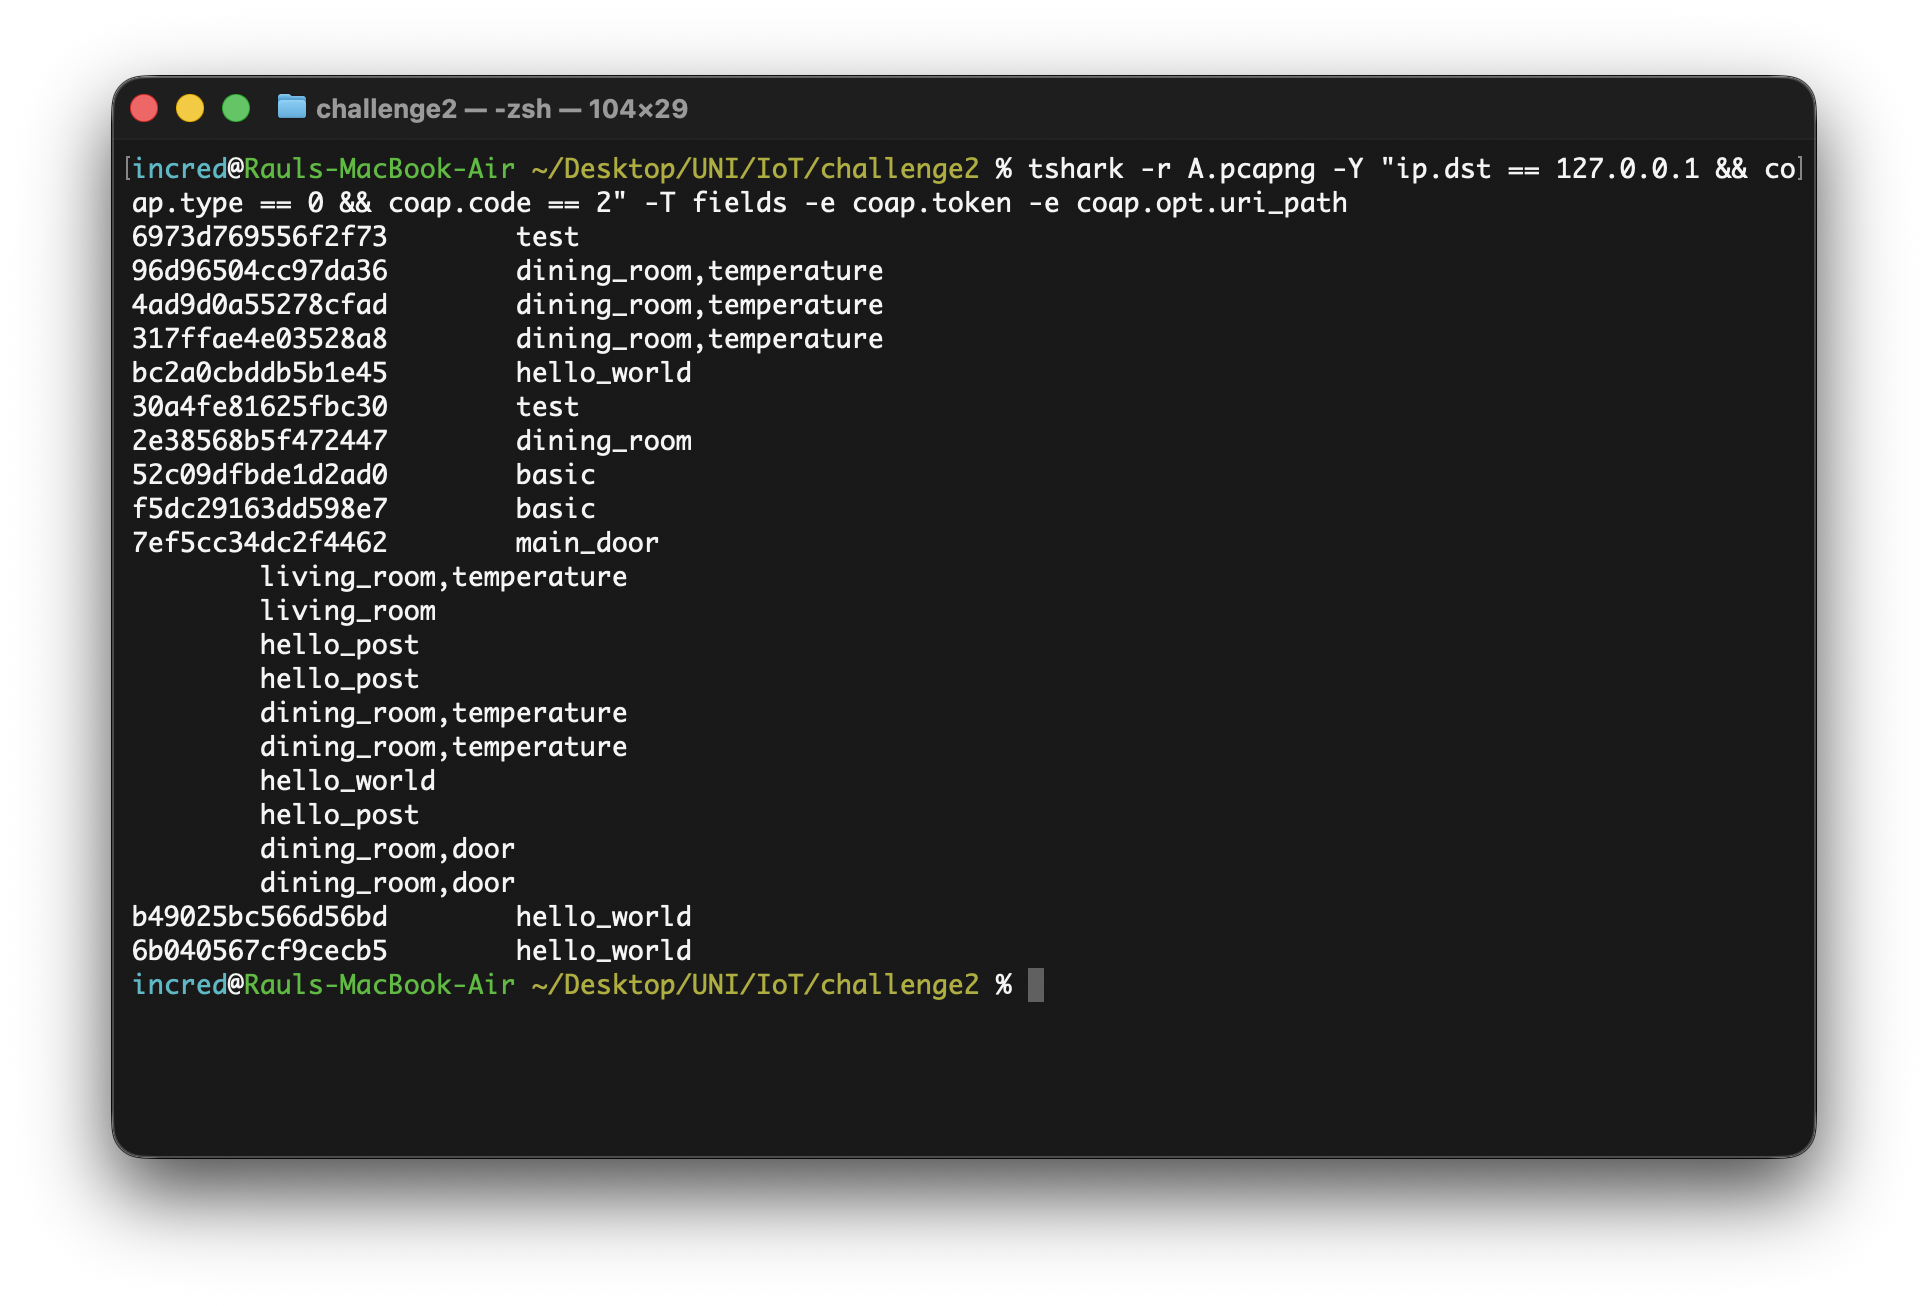
\includegraphics[width=\linewidth]{images/cq2-post.png}
        \vspace{0.1cm}\\
        Output saved in \textbf{\texttt{all\_post\_reqs.txt}}
    \end{minipage}\hfill
    \begin{minipage}[t]{0.48\textwidth}
        \textbf{Extract CON PUT requests:}
\begin{lstlisting}
ip.dst == 127.0.0.1 && 
coap.type == 0 && coap.code == 3
\end{lstlisting}
        \vspace{0.1cm}
        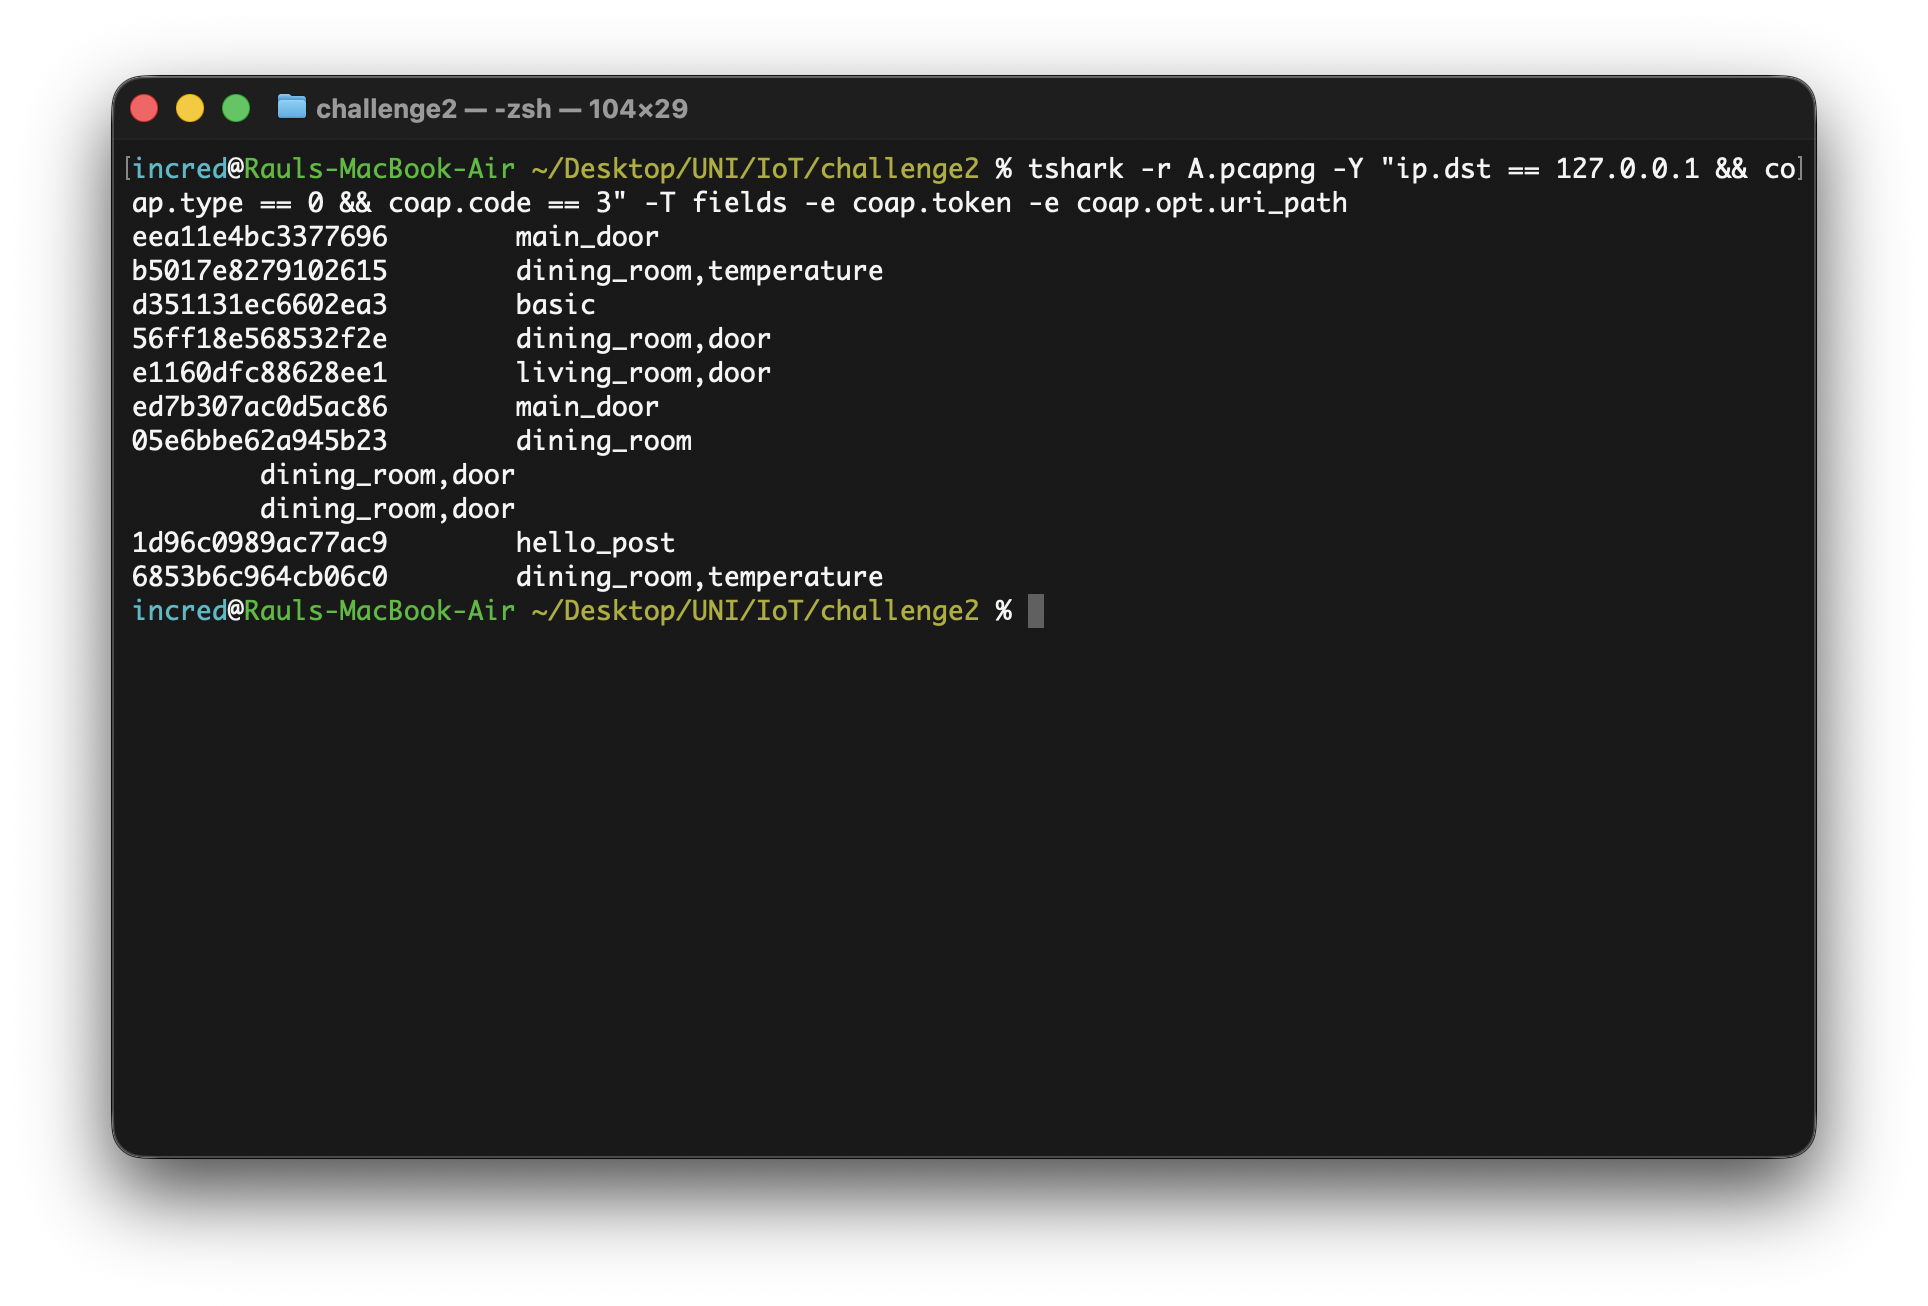
\includegraphics[width=\linewidth]{images/cq2-put.png}
        \vspace{0.1cm}\\
        Output saved in \textbf{\texttt{all\_put\_reqs.txt}}
    \end{minipage}
\end{figure}

\vspace{0.5cm}

\subsection*{Filter, Remove Duplicates and Count}
Identify which requests failed, count only unique requests, then add them by resource.

\begin{figure}[H]
    \centering
    \begin{minipage}[t]{0.48\textwidth}
        \subsubsection*{Find X (POST requests)}
\begin{lstlisting}
grep -f unsuccessful_tokens.txt all_post_reqs.txt | sort -u | awk '{print $2}' | sort | uniq -c | awk '{print $2, $1}' | sort > post_counts.txt
\end{lstlisting}
        \vspace{0.1cm}
        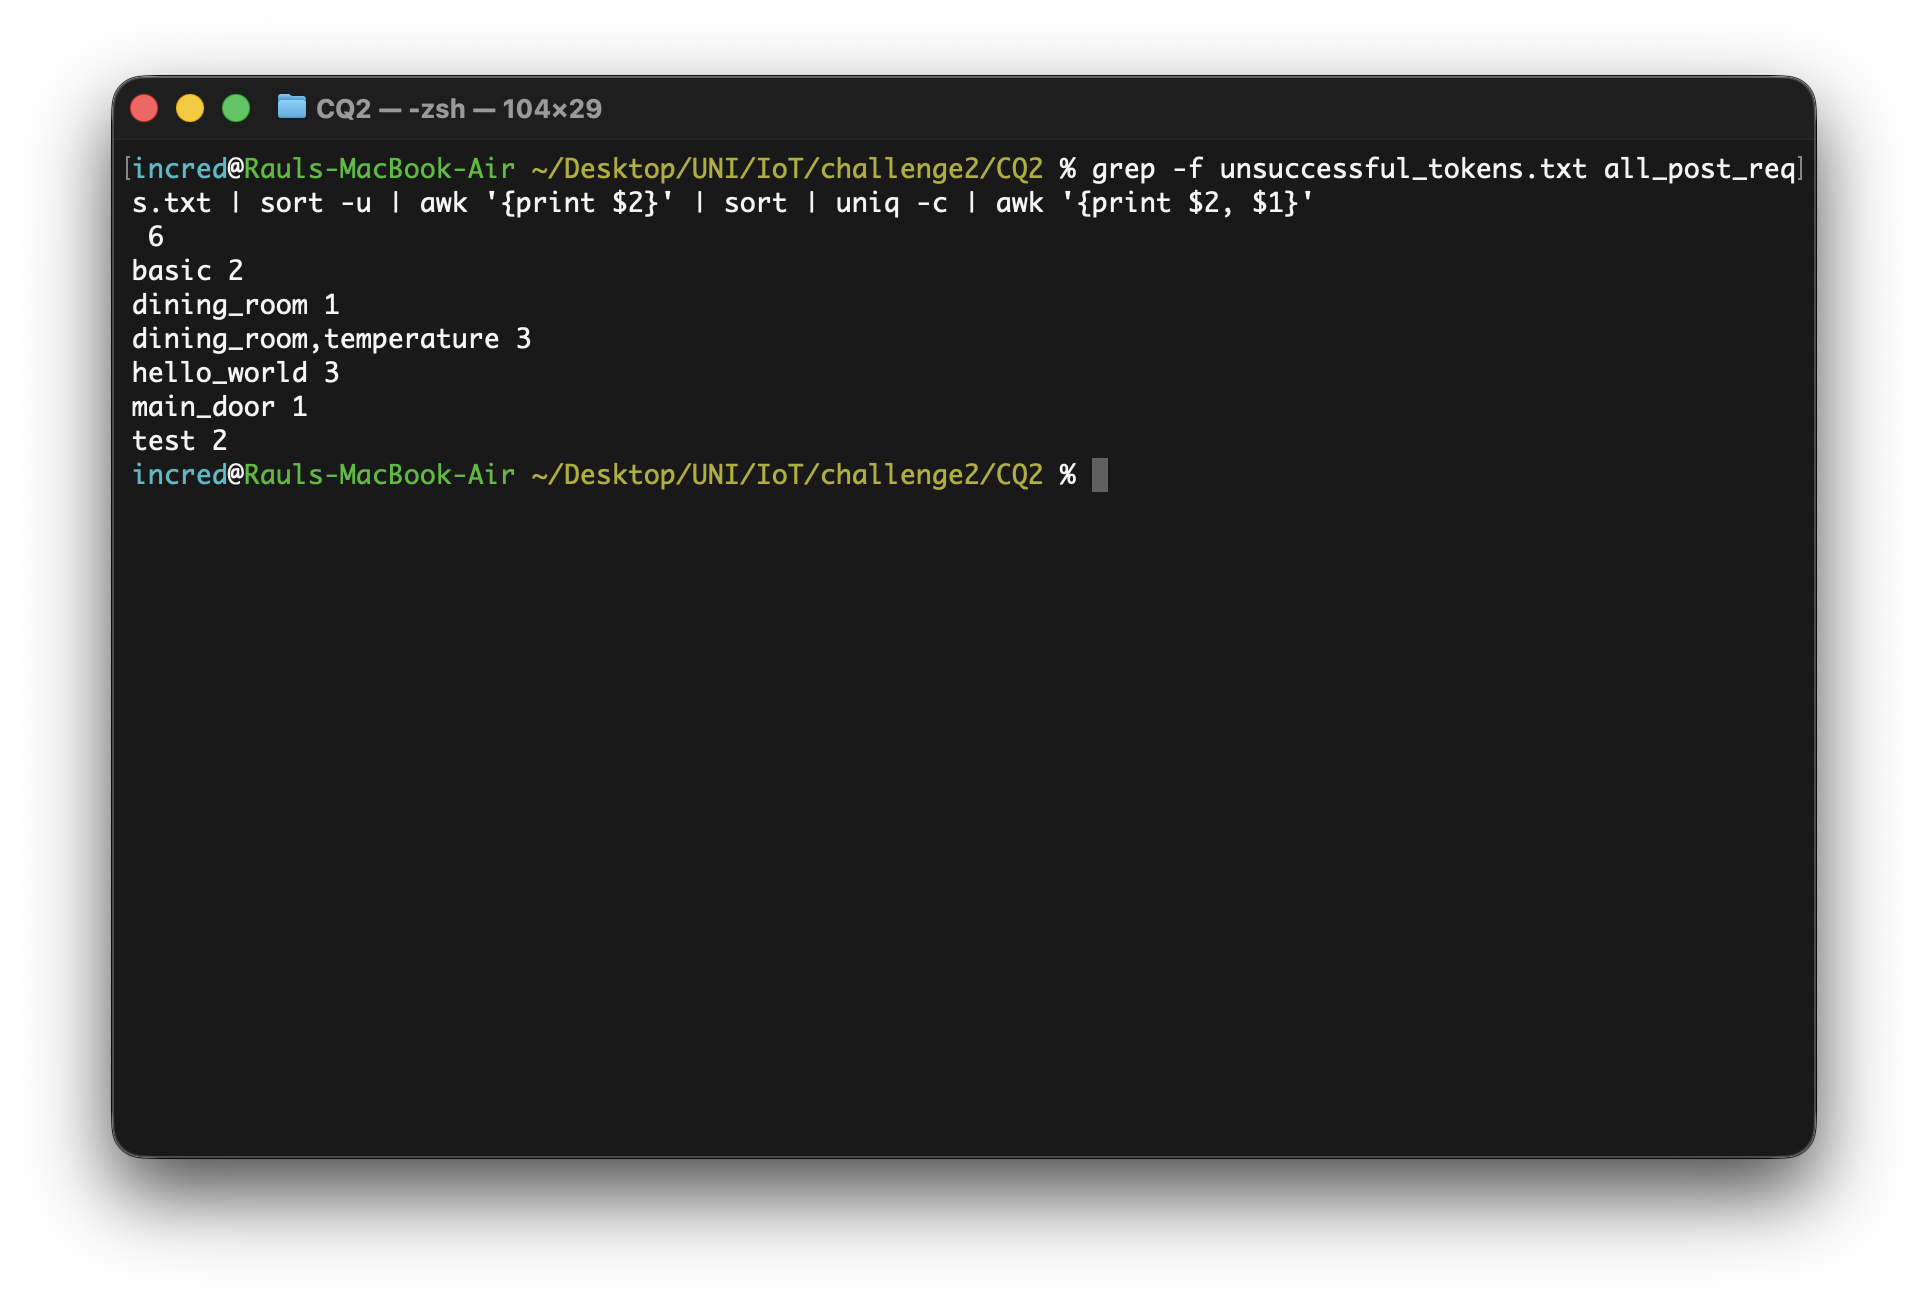
\includegraphics[width=\linewidth]{images/cq2-x.png}
        \vspace{0.1cm}\\
        Output saved in \textbf{\texttt{post\_counts.txt}}
    \end{minipage}\hfill
    \begin{minipage}[t]{0.48\textwidth}
        \subsubsection*{Find Y (PUT requests)}
\begin{lstlisting}
grep -f unsuccessful_tokens.txt all_put_reqs.txt | sort -u | awk '{print $2}' | sort | uniq -c | awk '{print $2, $1}' | sort > put_counts.txt
\end{lstlisting}
        \vspace{0.1cm}
        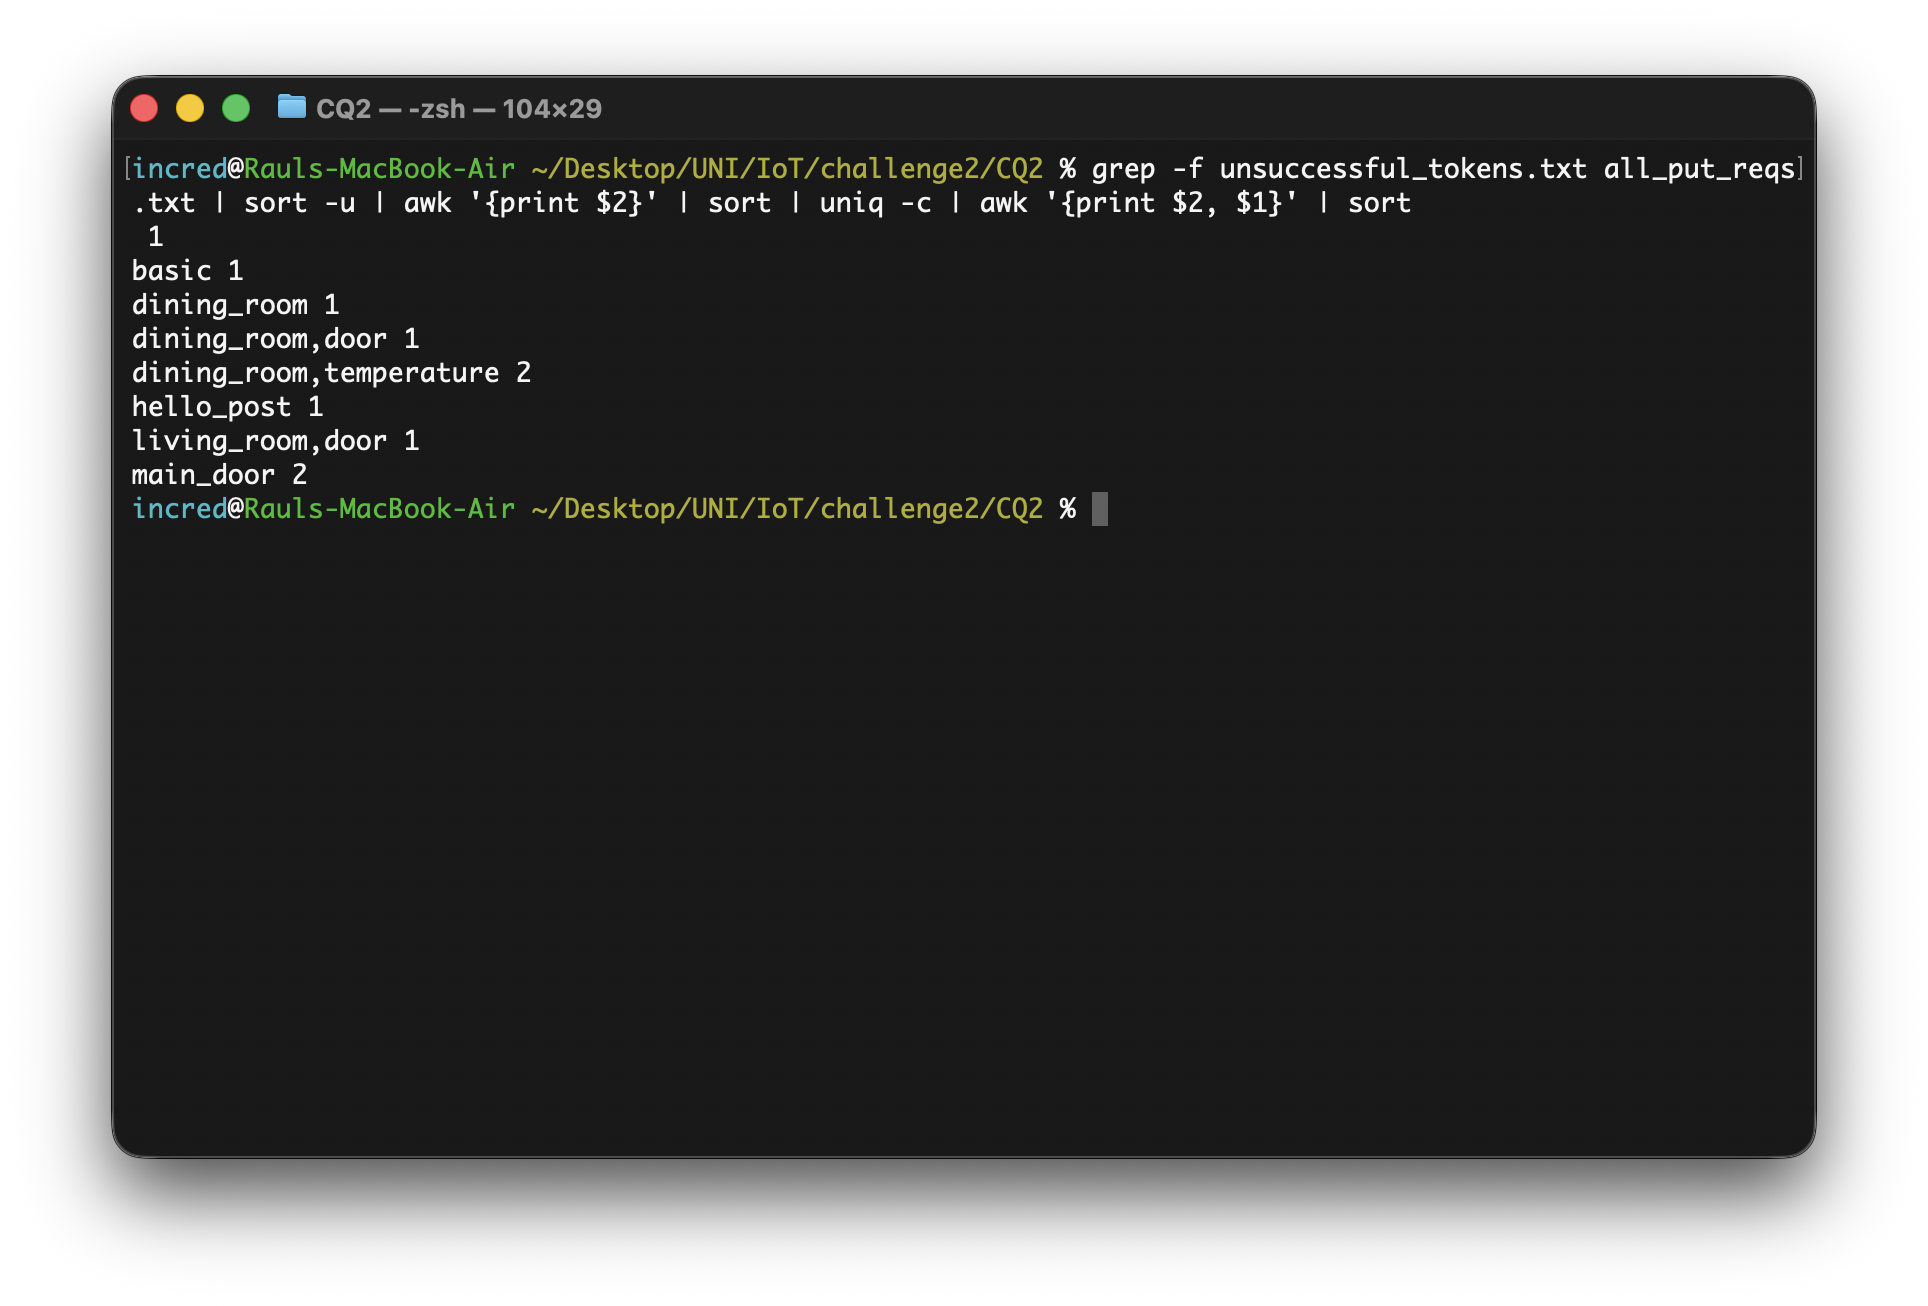
\includegraphics[width=\linewidth]{images/cq2-y.png}
        \vspace{0.1cm}\\
        Output saved in \textbf{\texttt{put\_counts.txt}}
    \end{minipage}
\end{figure}

\vspace{0.5cm}

\noindent
\begin{minipage}{\linewidth}
\subsection*{Compare the Results (Where $X = Y, X > 0$)}
Join the previous files together based on the resource name, check if the counts match, and verify that the count is greater than zero.
\begin{lstlisting}
join post_counts.txt put_counts.txt | awk '$2 == $3 && $2 > 0'
\end{lstlisting}

\begin{figure}[H]
    \centering
    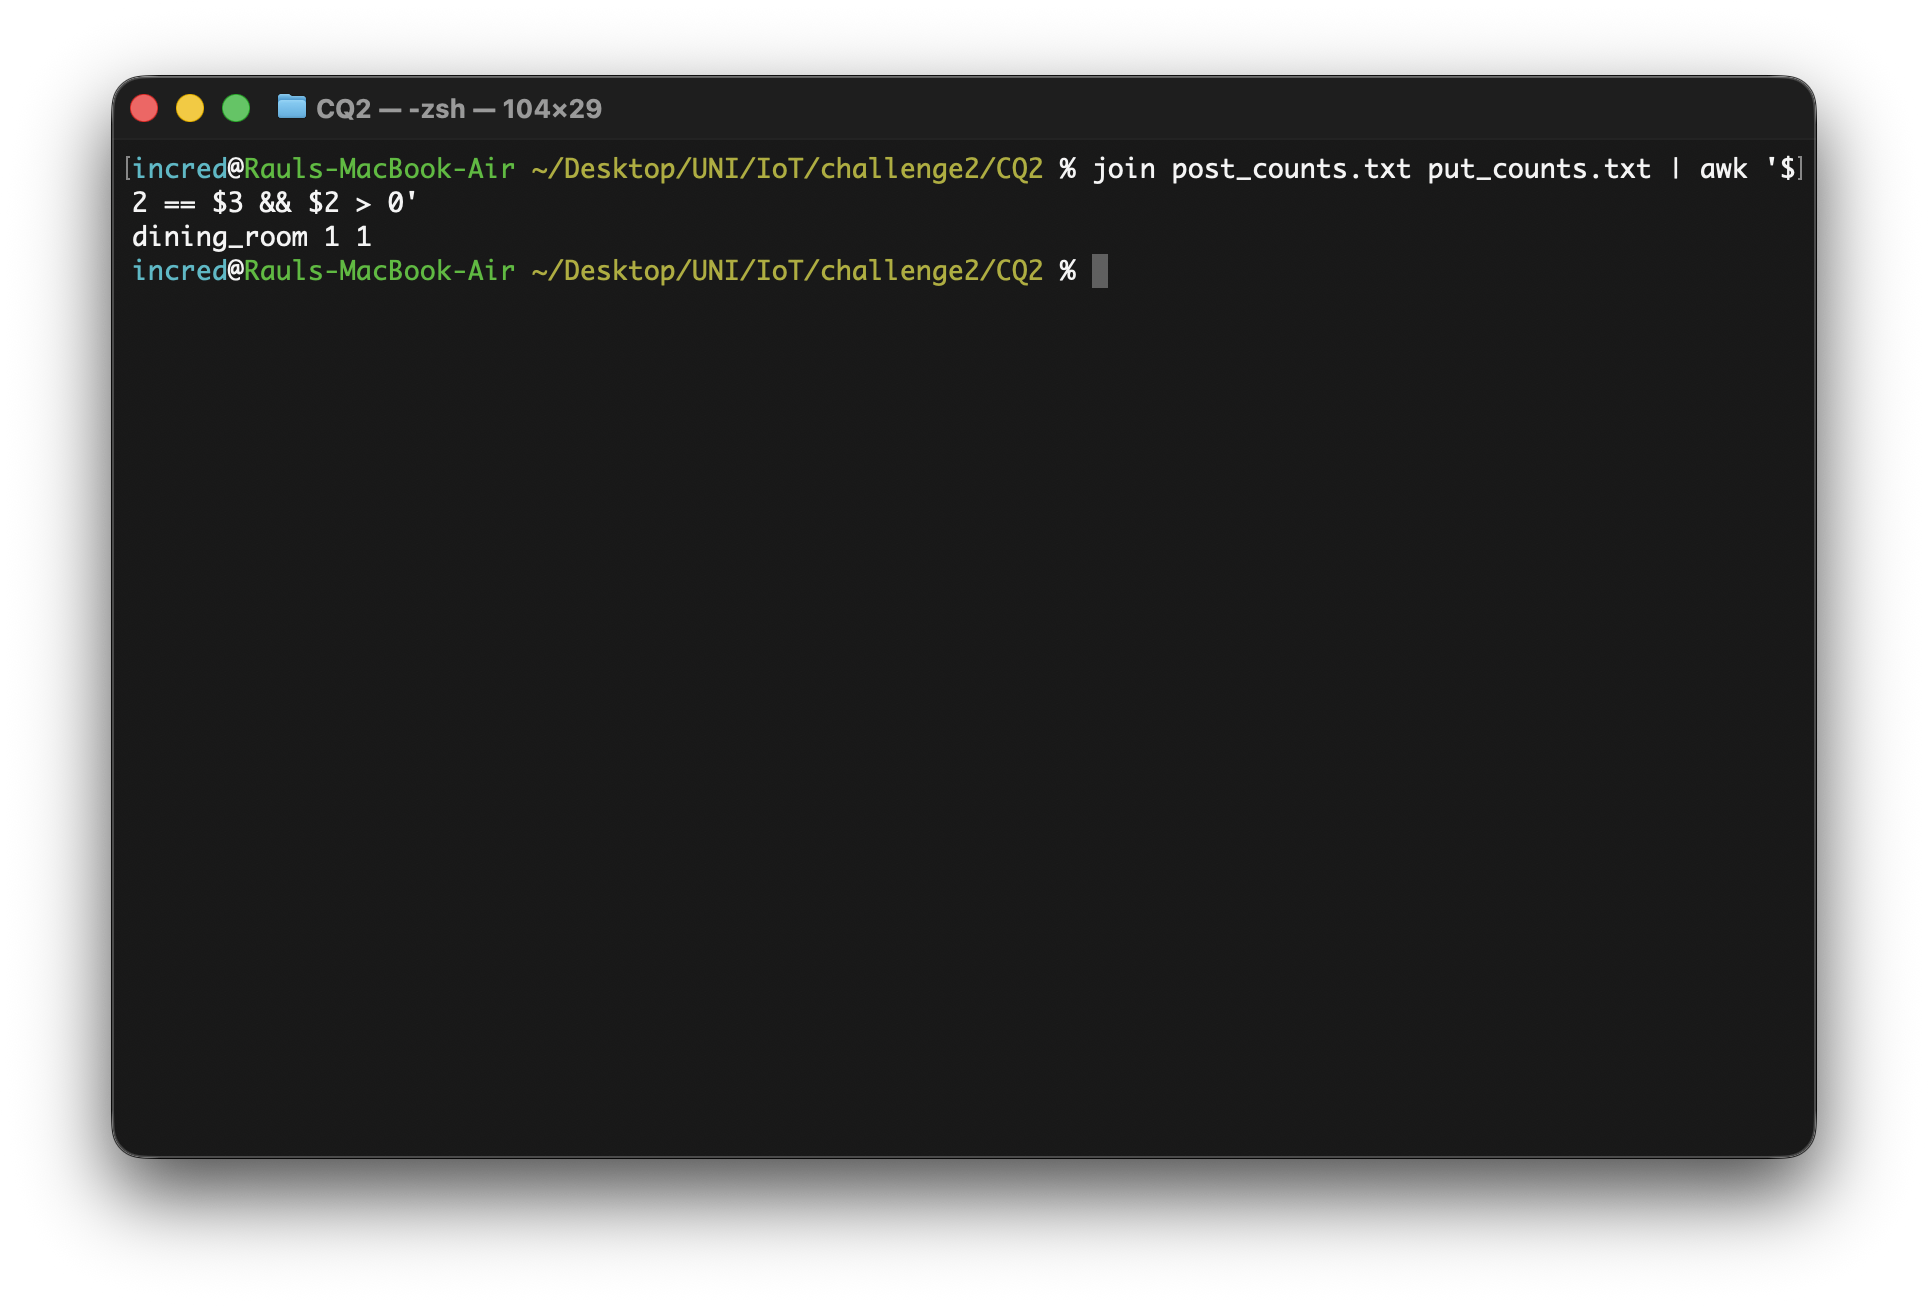
\includegraphics[width=0.75\linewidth]{images/cq2-result.png}
\end{figure}

\vspace{0.3cm}

\textbf{\huge Answer CQ2: 1}
\end{minipage}